\begin{tabular}{ c c  }
	\begin{tikzpicture}[scale=0.6]
		\begin{axis} [
			title = {\LARGE $\Hbarc{n}{\bbS^n}$},
			ticklabel style = {font=\Large},
			axis y line=middle,
			axis x line=middle,
			ytick={0.5,0.57,0.67,0.95},
			yticklabels={,$\zeta_n$,,$\pi$},
			xtick={0.5,0.57,0.95},
			xticklabels={$\frac{\pi}{2}$,$\zeta_n$, $\pi$},
			xmin=-0.015, xmax=1.1,
			ymin=0, ymax=1.1,]
			\addplot [thick,color=black!20!white,fill=black!30!white,
			fill opacity=0.4]coordinates {
				(0.57,0.95)
				(0.57,0.57)
				(0.95,0.95)
				(0.57,0.95)};
			\addplot [black!40!white,mark=none,dashed, thin] coordinates {(0,0.57) (0.57,0.57)};
			\addplot [black!40!white,mark=none,dashed, thin] coordinates {(0.57,0) (0.57,0.57)};
			\addplot[barccolor,mark=*] (0, 0.57) circle (2pt) node[above right,barccolor]{\Large\textsf{1}};
			\addplot [mark=none] coordinates {(0,0) (1,1)};
		\end{axis}
	\end{tikzpicture}
	&
	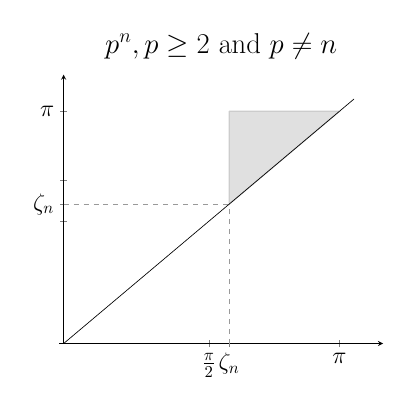
\begin{tikzpicture}[scale=0.6]
		\begin{axis} [
			title = {\LARGE $\Hbarc{p}{\bbS^n}, p\geq 2$ and $p\neq n$},
			ticklabel style = {font=\Large},
			axis y line=middle,
			axis x line=middle,
			ytick={0.5,0.57,0.67,0.95},
			yticklabels={,$\zeta_n$,,$\pi$},
			xtick={0.5,0.57,0.95},
			xticklabels={$\frac{\pi}{2}$,$\zeta_n$, $\pi$},
			xmin=-0.015, xmax=1.1,
			ymin=0, ymax=1.1,]
			\addplot [thick,color=black!20!white,fill=black!30!white,
			fill opacity=0.4]coordinates {
				(0.57,0.95)
				(0.57,0.57)
				(0.95,0.95)
				(0.57,0.95)};
			\addplot [black!40!white,mark=none,dashed, thin] coordinates {(0,0.57) (0.57,0.57)};
			\addplot [black!40!white,mark=none,dashed, thin] coordinates {(0.57,0) (0.57,0.57)};
			\addplot [mark=none] coordinates {(0,0) (1,1)};
		\end{axis}
	\end{tikzpicture}
\end{tabular}